% Options for packages loaded elsewhere
\PassOptionsToPackage{unicode}{hyperref}
\PassOptionsToPackage{hyphens}{url}
%
\documentclass[
  12pt,
]{article}
\usepackage{amsmath,amssymb}
\usepackage{lmodern}
\usepackage{iftex}
\ifPDFTeX
  \usepackage[T1]{fontenc}
  \usepackage[utf8]{inputenc}
  \usepackage{textcomp} % provide euro and other symbols
\else % if luatex or xetex
  \usepackage{unicode-math}
  \defaultfontfeatures{Scale=MatchLowercase}
  \defaultfontfeatures[\rmfamily]{Ligatures=TeX,Scale=1}
\fi
% Use upquote if available, for straight quotes in verbatim environments
\IfFileExists{upquote.sty}{\usepackage{upquote}}{}
\IfFileExists{microtype.sty}{% use microtype if available
  \usepackage[]{microtype}
  \UseMicrotypeSet[protrusion]{basicmath} % disable protrusion for tt fonts
}{}
\makeatletter
\@ifundefined{KOMAClassName}{% if non-KOMA class
  \IfFileExists{parskip.sty}{%
    \usepackage{parskip}
  }{% else
    \setlength{\parindent}{0pt}
    \setlength{\parskip}{6pt plus 2pt minus 1pt}}
}{% if KOMA class
  \KOMAoptions{parskip=half}}
\makeatother
\usepackage{xcolor}
\IfFileExists{xurl.sty}{\usepackage{xurl}}{} % add URL line breaks if available
\IfFileExists{bookmark.sty}{\usepackage{bookmark}}{\usepackage{hyperref}}
\hypersetup{
  hidelinks,
  pdfcreator={LaTeX via pandoc}}
\urlstyle{same} % disable monospaced font for URLs
\usepackage[margin=1in]{geometry}
\usepackage{longtable,booktabs,array}
\usepackage{calc} % for calculating minipage widths
% Correct order of tables after \paragraph or \subparagraph
\usepackage{etoolbox}
\makeatletter
\patchcmd\longtable{\par}{\if@noskipsec\mbox{}\fi\par}{}{}
\makeatother
% Allow footnotes in longtable head/foot
\IfFileExists{footnotehyper.sty}{\usepackage{footnotehyper}}{\usepackage{footnote}}
\makesavenoteenv{longtable}
\usepackage{graphicx}
\makeatletter
\def\maxwidth{\ifdim\Gin@nat@width>\linewidth\linewidth\else\Gin@nat@width\fi}
\def\maxheight{\ifdim\Gin@nat@height>\textheight\textheight\else\Gin@nat@height\fi}
\makeatother
% Scale images if necessary, so that they will not overflow the page
% margins by default, and it is still possible to overwrite the defaults
% using explicit options in \includegraphics[width, height, ...]{}
\setkeys{Gin}{width=\maxwidth,height=\maxheight,keepaspectratio}
% Set default figure placement to htbp
\makeatletter
\def\fps@figure{htbp}
\makeatother
\setlength{\emergencystretch}{3em} % prevent overfull lines
\providecommand{\tightlist}{%
  \setlength{\itemsep}{0pt}\setlength{\parskip}{0pt}}
\setcounter{secnumdepth}{-\maxdimen} % remove section numbering
\usepackage{float}
\usepackage{caption}
\usepackage{booktabs}
\usepackage{colortbl}
\usepackage{fancyhdr}
\pagestyle{fancy}
\usepackage[default]{sourcesanspro}
\usepackage{sourcecodepro}
\fancypagestyle{plain}{\pagestyle{fancy}}
\fancyhead[RE,RO]{Maenpuen \textit{et al}. --American Journal of Botany-- Appendix S3}
\ifLuaTeX
  \usepackage{selnolig}  % disable illegal ligatures
\fi

\author{}
\date{\vspace{-2.5em}}

\begin{document}

\hypertarget{appendix-s3}{%
\section{Appendix S3:}\label{appendix-s3}}

Generalization for a relationship between ratios of disc-based and whole-leaf-based estimates of leaf mass per area (LMA), leaf tissue density (LD), and leaf thickness (LT).
For the \emph{i} tree individual or species, the relationship between ratios of disc-based and whole-leaf estimates of LMA, LD, and LT is:

\[
\frac{\mathrm{LD_d}_i}{\mathrm{LD_w}_i} = \frac{\mathrm{LMA_d}_i}{\mathrm{LMA_w}_i} \frac{\mathrm{LT_w}_i}{\mathrm{LT_d}_i}
\]

where \emph{d} indicates disc-based estimates, \emph{w} indicates whole-leaf based estimates.

Because thickness is measured on leaf lamina whether one uses a leaf disc or a whole-leaf, the expected ratio between thickness for a leaf disc and a whole-leaf should be 1.
The above relationship, therefore, can be rewritten using lognormally distributed multiplicative error (\(\epsilon_i\)) on the arithmetic scale:

\[
\frac{\mathrm{LD_d}_i}{\mathrm{LD_w}_i} = \frac{\mathrm{LMA_d}_i}{\mathrm{LMA_w}_i} exp(\epsilon_i) \;\;\;\;\epsilon_i \sim \mathcal{N}(0, \sigma^2).
\]

LMA requires two times measurements (mass and area) and LD requires three time measurements (mass, area and thickness), and thus variance in the ratio of whole-leaf LD and leaf disc LD should be greater than that of LMA.

As we expected LD, showed the slightly smaller \emph{R}\textsuperscript{2} value than LMA (Figure below) in the Yunnan dataset.
We have independent measurement for thickness for leaf discs and whole-leaves in the Yunnan dataset.
If we use the same leaf thickness values for leaf discs and whole-leaves (i.e., LT\textsubscript{w\emph{i}}/LT\textsubscript{d\emph{i}} = 1), the scatter plots will be identical for LMA and LD.
Consequently, we do not perform further analyses for LD, because differences between whole-leaf LD and leaf disc LD only depends on the ratio between whole-leaf LMA and leaf disc LMA and measurement errors of leaf thickness.

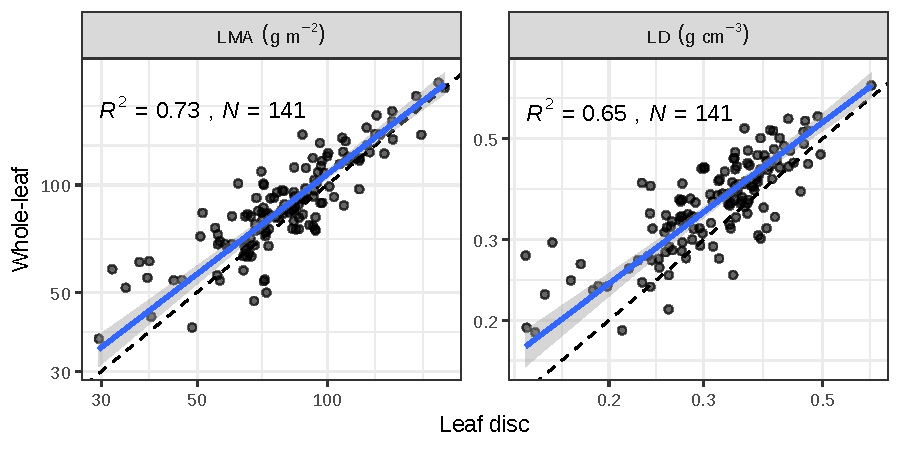
\includegraphics[width=6.25in,height=\textheight]{../figs/lma_ld.pdf}

Relationships between species mean leaf mass per area (LMA) and leaf tissue density (LD) determined by using whole leaves and leaf discs for the Yunnan dataset that has both leaf thickness for leaf discs and whole leaves.
Dashed lines indicate 1:1 lines.
Blue solid lines indicate standardized major axis regressions.
The 95\% confidence intervals are presented as the shaded area.
All the correlations are significant (\emph{P} \textless{} 0.001).

\end{document}
